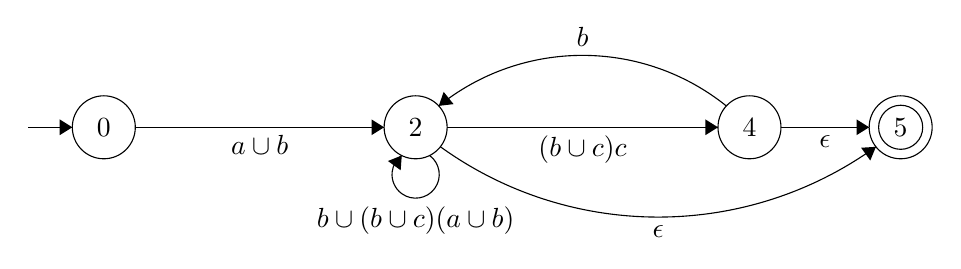
\begin{tikzpicture}[scale=0.2]
    \tikzstyle{every node}+=[inner sep=0pt]
    \draw [black] (5,-7) circle (2);
    \draw (5,-7) node {$0$};
    \draw [black] (24.8,-7) circle (2);
    \draw (24.8,-7) node {$2$};
    \draw [black] (46,-7) circle (2);
    \draw (46,-7) node {$4$};
    \draw [black] (55.6,-7) circle (2);
    \draw (55.6,-7) node {$5$};
    \draw [black] (55.6,-7) circle (1.4);
    \draw [black] (0.2,-7) -- (3,-7);
    \fill [black] (3,-7) -- (2.2,-6.5) -- (2.2,-7.5);
    \draw [black] (48,-7) -- (53.6,-7);
    \fill [black] (53.6,-7) -- (52.8,-6.5) -- (52.8,-7.5);
    \draw (50.8,-7.5) node [below] {$\epsilon$};
    \draw [black] (54.029,-8.237) arc (-54.20883:-125.79117:23.646);
    \fill [black] (54.03,-8.24) -- (53.09,-8.3) -- (53.67,-9.11);
    \draw (40.2,-13.2) node [below] {$\epsilon$};
    \draw [black] (25.682,-8.786) arc (54:-234:1.5);
    \draw (24.8,-12) node [below] {$b\cup (b\cup c)(a\cup b)$};
    \fill [black] (23.92,-8.79) -- (23.04,-9.14) -- (23.85,-9.73);
    \draw [black] (26.269,-5.645) arc (128.76337:51.23663:14.584);
    \fill [black] (26.27,-5.64) -- (27.21,-5.53) -- (26.58,-4.75);
    \draw (35.4,-1.93) node [above] {$b$};
    \draw [black] (7,-7) -- (22.8,-7);
    \fill [black] (22.8,-7) -- (22,-6.5) -- (22,-7.5);
    \draw (14.9,-7.5) node [below] {$a\cup b$};
    \draw [black] (26.8,-7) -- (44,-7);
    \fill [black] (44,-7) -- (43.2,-6.5) -- (43.2,-7.5);
    \draw (35.4,-7.5) node [below] {$(b\cup c)c$};
    \end{tikzpicture}